%%%%%%%%%%%%%%%%%%%%%%%%%%%%%
%% Styles, packages and new commands
\input{../Main/ML_Main.tex}
%%%%%%%%%%%%%%%%%%%%%%%%%%%%%
%% Edit the title page
\title{Machine Learning}
\subtitle{Module 5: Data Splitting}
\author[MOB]{Marc-Olivier Boldi}
\institute[HEC MSc Mgt BA]{Master in Management, Business Analytics, HEC UNIL}
\date[Spring 2024]{Spring 2024}
%%%%%%%%%%%%%%%%%%%%%%%%%%%%%
%%%%%%%%%%%%%%%%%%%%%%%%%%%%%
%%%%%%%%%%%%%%%%%%%%%%%%%%%%%
%%%%%%%%%%%%%%%%%%%%%%%%%%%%%
\begin{document}
%%%%%%%%%%%%%%%%%%%%%%%%%%%%%
\begin{frame}
  \titlepage
\end{frame}
%%%%%%%%%%%%%%%%%%%%%%%%%%%%%
\begin{frame}
\frametitle{Table of Contents}
	\tableofcontents
\end{frame}
%%%%%%%%%%%%%%%%%%%%%%%%%%%%%
%%%%%%%%%%%%%%%%%%%%%%%%%%%%%
\section{Concept}
%%%%%%%%%%%%%%%%%%%%%%%%%%%%%
%%%%%%%%%%%%%%%%%%%%%%%%%%%%%
\begin{frame}
\frametitle{Overfitting}
A good model should have the good metric (predictions) and a good capacity to extrapolate outside the data base. \\
\vspace{0.3cm}
Consider the following stupid but feasible model to predict an instance:
\begin{itemize}
\item if the instance is already in the data base, the predicted class is the same as the one in the data base.
\item if the instance is not already in the data base, the prediction is random.
\end{itemize}
The model will have a perfect accuracy on the data base. However, it is useless for new instances.
\end{frame}
%%%%%%%%%%%%%%%%%%%%%%%%%%%%%
\begin{frame}
\frametitle{Overfitting}
This example illustrates that it is easy to build good predictions when the data base is available: predicting the past is easy.\\
\vspace{0.3cm}
In the context of a supervised learning, a model may be good at predicting the data base on which it is trained but not the future/other data points. In practice however, this {\bf generalization capacity} is crucial.\\
\vspace{0.2cm}
A model having very good predictions on the data base, and a poor extrapolation capacity (for new instances) is said to {\bf overfit} the data.\\
\vspace{0.2cm}
{\bf Overfitting} is one of the worst enemy in machine learning: it looks like things are going well, when in fact no good new predictions can be obtained.
\end{frame}
%%%%%%%%%%%%%%%%%%%%%%%%%%%%%
%%%%%%%%%%%%%%%%%%%%%%%%%%%%%
\section{Training and test sets}
%%%%%%%%%%%%%%%%%%%%%%%%%%%%%
%%%%%%%%%%%%%%%%%%%%%%%%%%%%%
\begin{frame}
\frametitle{Concept}
The simplest data split consists of:
\begin{enumerate}
\item A {\bf training set} on which the models are trained;
\item A {\bf test set} on which predictions are tested.
\end{enumerate}
\end{frame}
%%%%%%%%%%%%%%%%%%%%%%%%%%%%%
\begin{frame}
\frametitle{Concept}
Often,
\begin{itemize}
\item The split is {\bf random} (assignment of the instances).
\item The two sets are {\bf disjoint}: no common instance, except if they are already multiple in the data base. 
\item Common proportions Tr/Te are like $75/25$ or $80/20$. 
\item However, with very large data base, it is useless to have too large training set. With millions of data points, often a $10\%$ training set is enough (if the data are representative and rich enough).
\end{itemize}
\end{frame}
%%%%%%%%%%%%%%%%%%%%%%%%%%%%%
\begin{frame}
\frametitle{Apparent and test metrics}
\begin{itemize}
\item On the training set, the metrics (accuracies, etc.) are called {\bf apparent metrics}: often too optimistic. 
\item The test set they are called {\bf test metrics}: close to the one expected when the model will be in use on new data.
\end{itemize}
To {\bf detect} overfitting, for a positive metric (e.g., accuracy),
\begin{itemize}
\item If $Metric(Tr) >> Metric(Te)$: overfitting.
\item If $Metric(Tr) \approx Metric(Te)$: no sign of overfitting.
\end{itemize}
\end{frame}
%%%%%%%%%%%%%%%%%%%%%%%%%%%%%
\begin{frame}[fragile]
\frametitle{Example}
A data set with 1000 instances,
\begin{itemize}
\item Split at random: 
\begin{itemize}
\item training set of 750 instances,
\item Test set of 250 instances. 
\end{itemize}
\item A logistic regression is fitted to the training set. 
\item The features of the test set are given to the model to make the test set predictions. These are compared to the correct classes in the test set. 
\item The apparent (left) and test (right) confusion matrices:\\
\scriptsize
\begin{columns}
\begin{column}{0.5\textwidth}
\begin{verbatim}
          Reference
Prediction Bad Good
      Bad   30   19
      Good 195  506
\end{verbatim}
\end{column}
\begin{column}{0.5\textwidth}
\begin{verbatim}
          Reference
Prediction Bad Good
      Bad    6    7
      Good  69  168
\end{verbatim}
\end{column}
\end{columns}
\normalsize
\end{itemize}
\end{frame}
%%%%%%%%%%%%%%%%%%%%%%%%%%%%%
\begin{frame}
\frametitle{Example}
The apparent and test accuracies are
$$
A_{tr} = \frac{30+506}{750} = 0.715, \quad
A_{te} = \frac{6+168}{250} = 0.696.
$$
The accuracy on the test set is closer to the one that can be expected if the model was used on new instances (e.g., in production).\\
\vspace{0.3cm}
Here, the test accuracy is lower than the apparent accuracy. This is a usual sign of over-fitting\footnote{Mild though.}.
\end{frame}
%%%%%%%%%%%%%%%%%%%%%%%%%%%%%
%%%%%%%%%%%%%%%%%%%%%%%%%%%%%
\section{Validation set}
%%%%%%%%%%%%%%%%%%%%%%%%%%%%%
%%%%%%%%%%%%%%%%%%%%%%%%%%%%%
\begin{frame}
\frametitle{Validation set}
When the training set is split further into a training set\footnote{There is no specific name to distinguish between the first ``big'' training set, and the second one, that is smaller.} and a {\bf validation set}.
\begin{itemize}
\item Several models are trained on this smaller training set
\item The best model is selected based on the metrics obtained on the validation set.
\item The test metric of best model is computed to have a final evaluation of what this metric will be on new data.
\end{itemize}
This avoids {\bf information leakage}: selecting the best model on the test set may cause overfitting of this test set...\\
\vspace{0.3cm}
Validation set is also used for cross-validation, hyperparameter selection, early stopping, etc. See below.
\end{frame}
%%%%%%%%%%%%%%%%%%%%%%%%%%%%%
\begin{frame}
\frametitle{Illustration}
\begin{center}
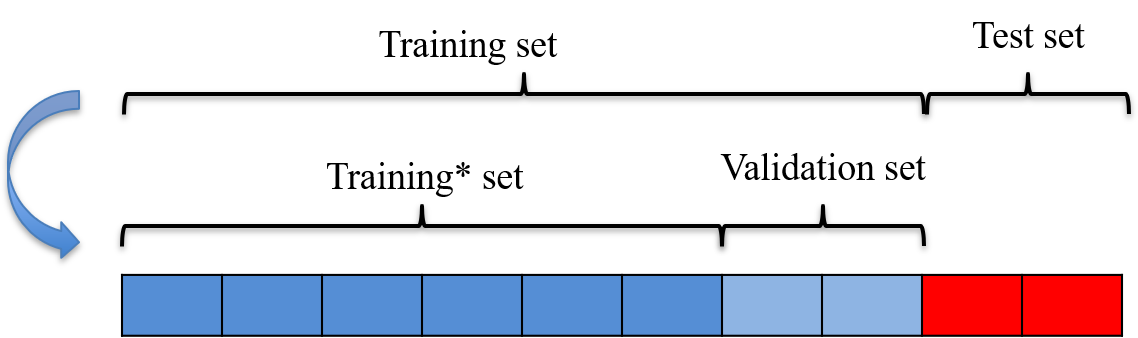
\includegraphics[width=8cm]{../Graphs/Validation_set.png}
\end{center}
\end{frame}
%%%%%%%%%%%%%%%%%%%%%%%%%%%%%
\section{Repeated splits}
%%%%%%%%%%%%%%%%%%%%%%%%%%%%%
\begin{frame}
\frametitle{Repeated splits}
One single training/validation/test split taken at random can be unstable or impossible to replicate: the randomness was badly balanced or too much dependence on this specific split.\\ 
\vspace{0.3cm}
{\bf Repeated splits} can be used to address this issue. They are under two forms:
\begin{itemize}
\item {\bf Cross-validation} (CV).
\item {\bf Bootstrap}.
\end{itemize}
\end{frame}
%%%%%%%%%%%%%%%%%%%%%%%%%%%%%
\begin{frame}
\frametitle{$K$-fold CV}
\begin{enumerate}
\item Split the data set into non-overlapping $K$ subsets, 
\item For each $k=1,\ldots,K$, 
\begin{itemize}
\item Use subset $k$ as the validation set, and the rest of the data set as the training set,
\item Train the model on the training set
\item Compute the predictions on the validation set
\item Compute and record the metric $S_k$ 
\end{itemize}
\end{enumerate}
This provides $K$ metrics: $S_1, \ldots, S_K$. The final CV metric is their average:
$$
\hat{S} = \frac{1}{K}\sum_{k=1}^K S_k.
$$
In addition, these metrics are used to estimate the standard deviation\footnote{Technically, this is the method used in 1-SE rule for trees.} of $\hat{S}$. 
\end{frame}
%%%%%%%%%%%%%%%%%%%%%%%%%%%%%
\begin{frame}
\frametitle{$K$-fold CV}
\begin{center}
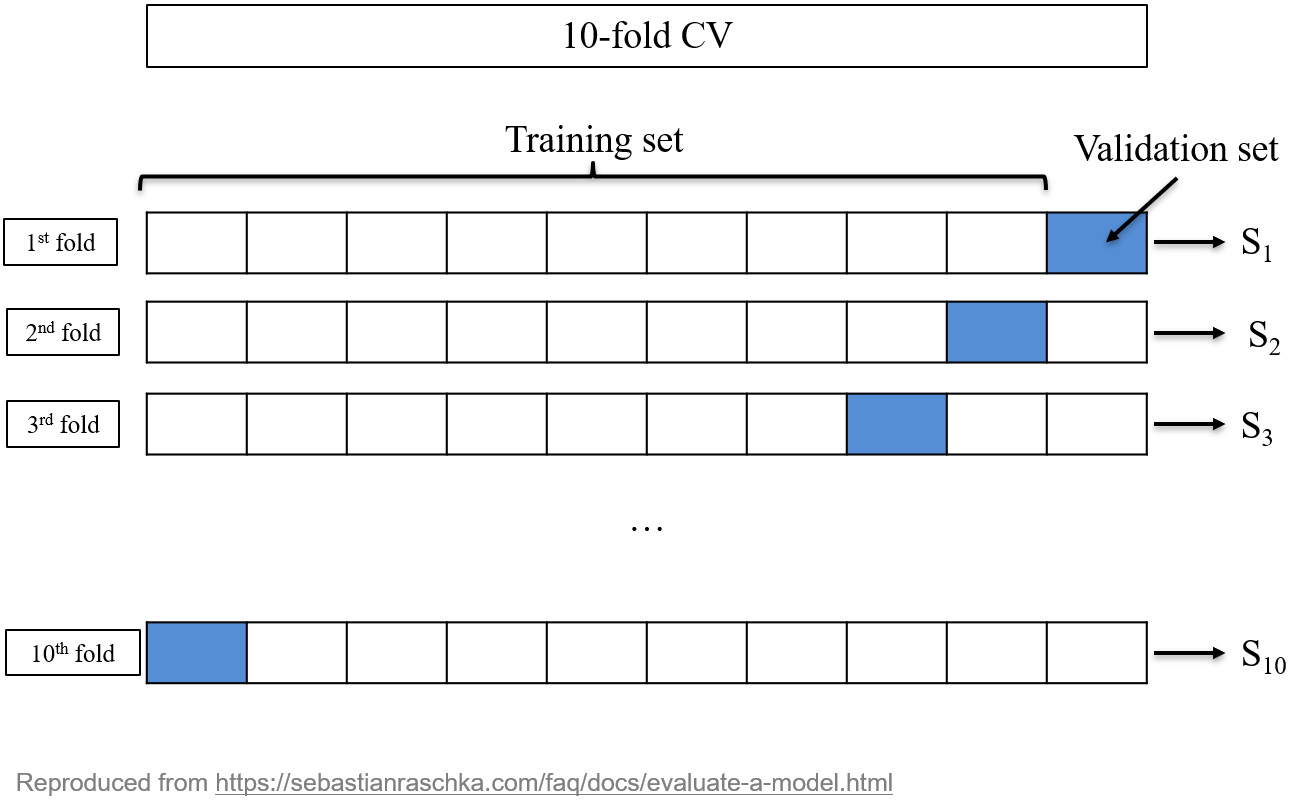
\includegraphics[width=10cm]{../Graphs/10-CV.png}
\end{center}
\end{frame}
%%%%%%%%%%%%%%%%%%%%%%%%%%%%%
\begin{frame}
\frametitle{Example}
A 10-fold CV is made. The accuracies of are logistic regression in each fold are
$$
\begin{array}{|c|c|c|c|c|c|c|c|c|c|}
\hline
S_1 & S_2 & S_3 & S_4 & S_5 & S_6 & S_7 & S_8 & S_9 & S_{10}\\
\hline
0.63 & 0.71 & 0.73 & 0.73 & 0.76 & 0.64 & 0.71 & 0.75 & 0.78 & 0.69\\
\hline
\end{array}
$$
The CV accuracy (standard deviation) is $0.713$ $(0.049)$.\\
\vspace{0.3cm}
On the same data split, another model gives CV accuracy of 0.654 (0.053).\\ 
\vspace{0.3cm}
The logistic regression should be preferred here.
\end{frame}
%%%%%%%%%%%%%%%%%%%%%%%%%%%%%
\begin{frame}
\frametitle{$K$-fold CV}
\begin{center}
How to choose $K$?
\end{center}
\begin{itemize}
\item No universal good choice.
\item Choice of $K$ is a trade-off between 
\begin{itemize}
\item computational capacity: large $K$ gives more iterations and larger training sets, thus longer computation.
\item number of validation metrics: large $K$ gives more $S_k$ so $\hat{S}$ is well estimated.
\item number of data to train the model: large $K$ gives large training set thus better estimated models.
\item number of data to estimate the validation metric: large $K$ gives small validation set, thus $S_k$ is not well estimated.
\end{itemize}
\item In practice, use $K=5$ or $K=10$.\\
\item A special case is $K=n$, known as {\bf leave-one-out} (LOO). \\
\end{itemize} 
\end{frame}
%%%%%%%%%%%%%%%%%%%%%%%%%%%%%
\begin{frame}
\frametitle{Bootstrap: Re-sampling}
In context of ML, {\bf bootstrap} stands for {\bf re-sampling with replacement}. It is an alternative to CV. The differences between CV and bootstrap are
\begin{itemize}
\item for CV, the whole data base is split once. Training and validation sets do not have common instances.
\item For bootstrap, the training and validation sets vary in size and composition at each step. 
\end{itemize}
The fact that instances can be repeated in the training set can create a bias. A weighted estimate tackles this issue: the {\bf 632-rule}. 
\end{frame}
%%%%%%%%%%%%%%%%%%%%%%%%%%%%%
\begin{frame}
\frametitle{Bootstrap: Procedure}
In practice, one bootstrap step consists of
\begin{enumerate}
\item Select at random a training set by sampling from the original data base, {\it with replacements}, a training set {\it of the same size}.
\item The instances in the original data base {\it that are not in the generated training set} constitute the validation set. 
\item Compute the metric on the validation set after having trained the model with the training set: {\bf out-of-bag} metric, $\hat{S}_{oob}$.
\item Compute also the prediction of the training set itself: {\bf apparent} metric, $\hat{S}_{app}$.
\item Estimate the metric using the {\bf 632-rule}:
$$
\hat{S} = 0.632 \times \hat{S}_{oob} + 0.368 \times \hat{S}_{app}.
$$
\end{enumerate}
\end{frame}
%%%%%%%%%%%%%%%%%%%%%%%%%%%%%
\begin{frame}
\frametitle{One bootstrap step}
\begin{center}
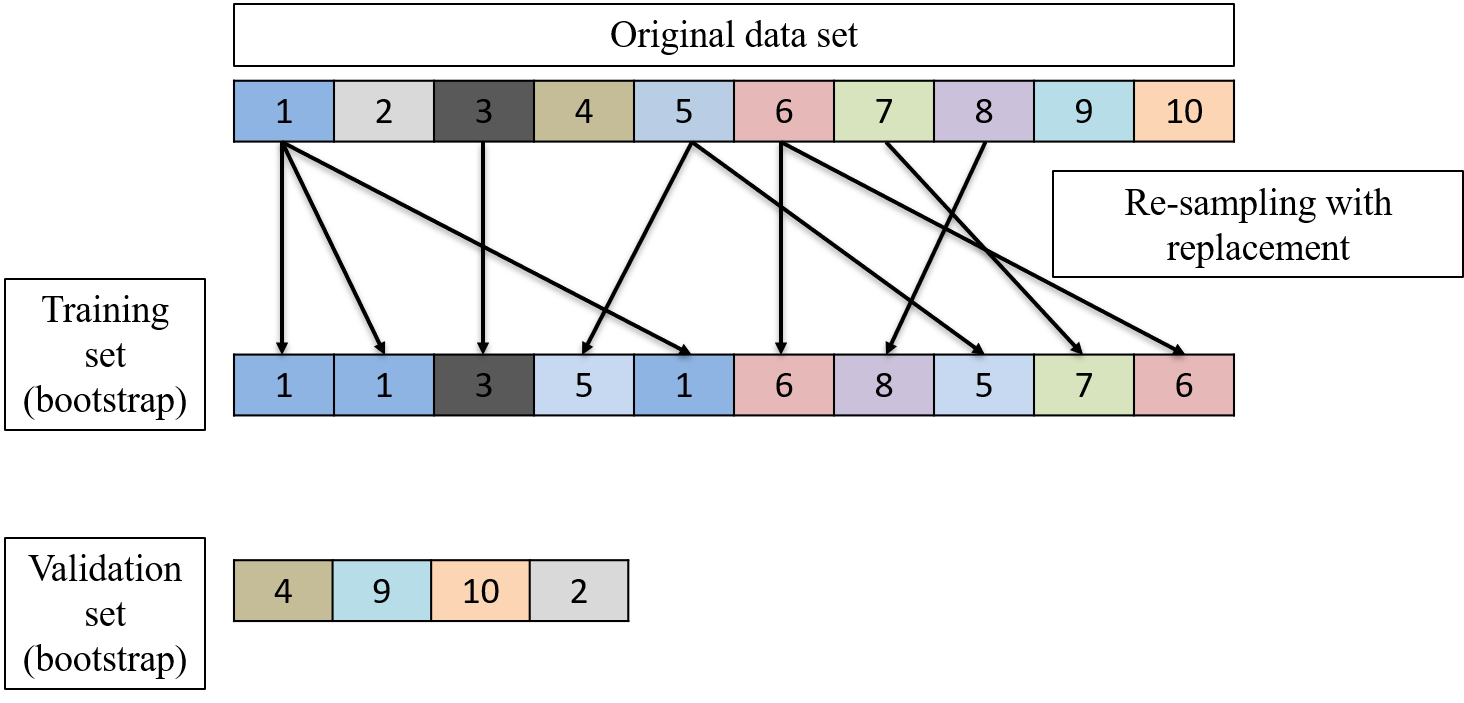
\includegraphics[width=11cm]{../Graphs/Bootstrap.png}
\end{center}
\end{frame}
%%%%%%%%%%%%%%%%%%%%%%%%%%%%%
\begin{frame}
\frametitle{Bootstrap estimate}
The previous bootstrap step is repeated a large number of times; typically 500 to 10'000, depending on the time it takes (computation power).\\ 
\vspace{0.3cm}
The final estimate is the average of each $\hat{S}$. Standard deviation can be also computed.\\
\vspace{0.3cm}
\end{frame}
%%%%%%%%%%%%%%%%%%%%%%%%%%%%%
\begin{frame}
\frametitle{Bootstrap samples}
\begin{center}
How many bootstrap samples ($R$) should be used?
\end{center} 
\begin{itemize}
\item There is no theoretical number but people consider that it should be at least large enough so that all the instances of the data base are at least once selected in a validation set.
\item In general, a large number, depending on the computational power and the data set size. 
\end{itemize}
\end{frame}
%%%%%%%%%%%%%%%%%%%%%%%%%%%%%
\begin{frame}
\frametitle{Practical use}
\begin{itemize}
\item With small data base, prefer bootstrap.
\item With large data base, prefer CV.
\item CV can be repeated: several CV pattern are simulated independently and aggregated at the end. 
\item These procedures can be computed in parallel for better performance.
\end{itemize}
\end{frame}
%%%%%%%%%%%%%%%%%%%%%%%%%%%%%
%%%%%%%%%%%%%%%%%%%%%%%%%%%%%
\section{Solving the overfitting problem}
%%%%%%%%%%%%%%%%%%%%%%%%%%%%%
%%%%%%%%%%%%%%%%%%%%%%%%%%%%%
\begin{frame}
\frametitle{Solving overfitting}
Comparing apparent and test metrics allows to detect overfitting only. How can we improve the situation?\\
\vspace{0.3cm}
A model that overfits the training data set is too flexible/complex. We can use the methods seen for each model to try to simplify them:
\begin{itemize}
\item Linear and logistic regression: variable selection and/or use $L_1$ and $L_2$ penalization.
\item Trees: prune the tree.
\item SVM: tune the cost parameter and/or the parameters of the kernel.
\item NN: use $L_1$ and $L_2$ penalization and/or simplify the structure of the network.
\end{itemize}

\end{frame}
%%%%%%%%%%%%%%%%%%%%%%%%%%%%%
\begin{frame}
\frametitle{Hyperparameters}
Some of these methods require to set parameters: penalization parameter, cost parameter, others.\\ 
\vspace{0.3cm}
These are called {\bf hyperparameters}.Hyperparameters are structural parameters or "pseudo-parameters" of the models.\\
\vspace{0.3cm}
An informal definition is "whatever cannot be optimized by the training algorithm".\\
\vspace{0.3cm}
To set these parameters is called {\bf tuning}.
\end{frame}
%%%%%%%%%%%%%%%%%%%%%%%%%%%%%
\begin{frame}
\frametitle{Tuning hyperparameters}
The main technique consists of direct comparison (brute force):
\begin{itemize}
\item Create a list of possible hyperparameter values. 
\item Train all the models from the list.
\item Select the best in class according to the validation metric.
\end{itemize}
This approach can be done on
\begin{itemize}
\item A simple split: training and validation
\item A repeated split: bootstrap or CV.
\end{itemize}
The choice of the hyperparameters must not be done on the test: a part of the information contained in the test set may {\it leaks} to the model choice and thus to the training.\\ 
\vspace{0.3cm}
Avoid any {\bf information leakage}: the {\bf test set must not be seen} by the model, at any stage.
\end{frame}
%%%%%%%%%%%%%%%%%%%%%%%%%%%%%
\section{Solving the unbalance problem}
%%%%%%%%%%%%%%%%%%%%%%%%%%%%%
\begin{frame}[fragile]
\frametitle{Unbalanced classes}
"Unbalanced classes" refers to data set where the classes frequencies are unbalanced. E.g., doctor visit data have 4 times more ``No'' than ``Yes''.\\
\scriptsize
\begin{verbatim}
  No  Yes 
4141 1049
\end{verbatim}
\normalsize
During the training, the model favors the predictions of the ``No'' to reach a better accuracy. 
\end{frame}
%%%%%%%%%%%%%%%%%%%%%%%%%%%%%
\begin{frame}[fragile]
\frametitle{Unbalanced classes}
E.g., the logistic regression, gives:\\
\scriptsize
\begin{verbatim}
Confusion Matrix and Statistics
[...]
               Accuracy : 0.8091          
[...]                                          
            Sensitivity : 0.9771          
            Specificity : 0.1435          
[...]
      Balanced Accuracy : 0.5603
\end{verbatim}
\normalsize
This problem is {\bf detected} with
\begin{itemize}
\item low balanced accuracy
\item low sensitivity or specificity
\end{itemize}
\end{frame}
%%%%%%%%%%%%%%%%%%%%%%%%%%%%%
\begin{frame}
\frametitle{Tuning probability threshold}
One approach to solve this issue is to tune the probability threshold $\lambda$:
$$
f(x_i;\theta) = \left\{
\begin{array}{ll}
1, & \mbox{if } p(x_i;\theta) > \lambda,\\
0, & \mbox{if } p(x_i;\theta) \leq \lambda.
\end{array}
\right.
$$
To maximize the balanced accuracy, find the threshold $\lambda$ that maximizes the {\bf Youden's J statistics}:
$$
J(\lambda) = \mbox{Spec}(\lambda) + \mbox{Sens}(\lambda) - 1.
$$
Note: this optimization is always at at cost of a lower accuracy.
\end{frame}
%%%%%%%%%%%%%%%%%%%%%%%%%%%%%
\begin{frame}[fragile]
\frametitle{Tuning probability threshold}
Example after optimization:\\
\scriptsize
\begin{verbatim}
Confusion Matrix and Statistics
[...]                     
               Accuracy : 0.6991          
[...]
            Sensitivity : 0.7186          
            Specificity : 0.6220          
[...]
      Balanced Accuracy : 0.6703  
\end{verbatim}
\normalsize
Sensitivity decreased, specificity increased. Overall BA increased (and accuracy decreased).\\
\vspace{0.3cm}
{\bf The probability threshold $\lambda$ is an hyperparameter}. Use the splitting data method to avoid overfitting.
\end{frame}
%%%%%%%%%%%%%%%%%%%%%%%%%%%%%
\begin{frame}
\frametitle{Class balancing}
Another approach consists of {\bf balancing} the classes {\it in the training set}. Two possible approaches:
\begin{itemize}
\item {\bf Sub-sampling}: Remove cases in the training set,
\item {\bf Re-sampling}: Add cases in the training set.
\end{itemize}
\begin{center}
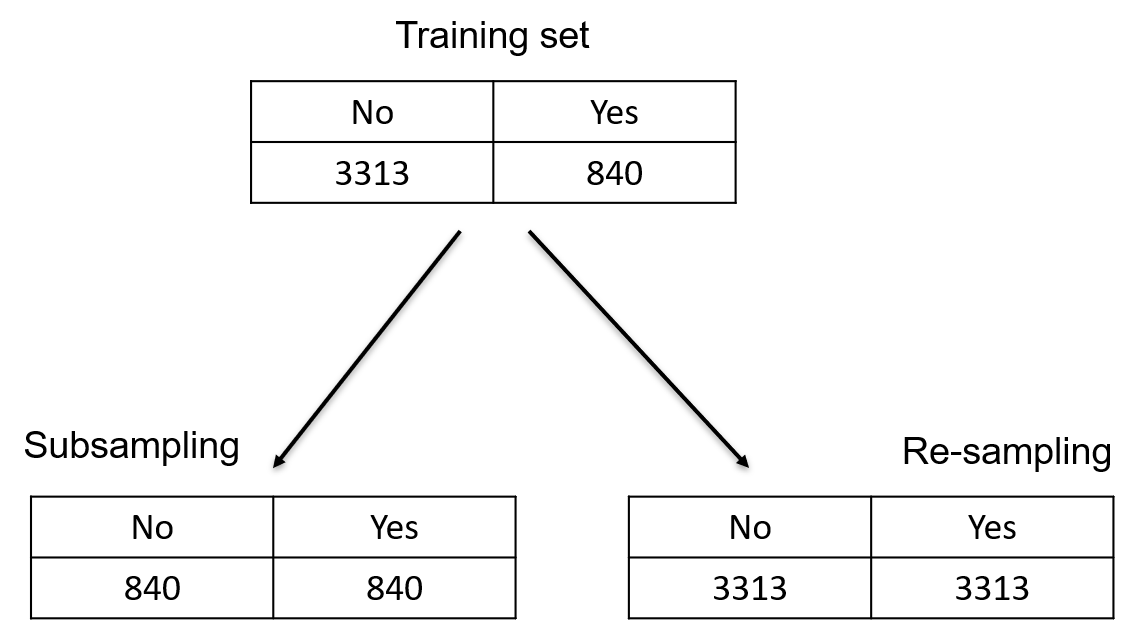
\includegraphics[width=6cm]{../Graphs/Balancing.png}
\end{center}
\end{frame}
%%%%%%%%%%%%%%%%%%%%%%%%%%%%%
\begin{frame}
\frametitle{Class balancing}
In details
\begin{itemize}
\item Sub-sampling: take all the ``Yes'' and a random subset of ``No'' of the same size.
\item Re-sampling: take all the ``No'' and add replicates of the ``Yes'', chosen at random, until there are as many ``Yes'' as ``No''.
\end{itemize}
Variations are possible to increase or decrease the weight of each class, to take into account for the proportions.\\
\vspace{0.3cm}
Note: {\bf the test set must NOT be balanced}.
\end{frame}
%%%%%%%%%%%%%%%%%%%%%%%%%%%%%
\begin{frame}[fragile]
\frametitle{Class balancing}
Example,\\
\vspace{0.2cm}
\scriptsize
With sub-sampling
\begin{verbatim}
               Accuracy : 0.7049          
[...]
            Sensitivity : 0.7331          
            Specificity : 0.5933          
[...]
      Balanced Accuracy : 0.6632          
\end{verbatim}
With re-sampling
\begin{verbatim}
               Accuracy : 0.7097       
[...]
            Sensitivity : 0.7391          
            Specificity : 0.5933          
[...]
      Balanced Accuracy : 0.6662          
\end{verbatim}
The results are similar to tuning of $\lambda$.
\end{frame}
%%%%%%%%%%%%%%%%%%%%%%%%%%%%%
\begin{frame}
\frametitle{Discussion on class balancing}
\begin{itemize}
\item Case imbalance is a common problem in real life data (fraud detection, rare events, etc.).
\item Applied on the data, class balancing is a possible solution to improve the fit.
\item Unlike tuning of the probability threshold, class balancing can be apply to no-probability models and multi-class problems.
\item There is no guarantee. The final performances must be inspected.
\item {\bf The test set must remain unbalanced} to be representative of future data.
\item If you use CV or bootstrap, the validation set must remain unbalanced (often not the case in built-in methods). 
\end{itemize}
\end{frame}
%%%%%%%%%%%%%%%%%%%%%%%%%%%%%
\end{document}

\begin{frame}[fragile]
\frametitle{Unbalanced classes}
Unbalanced classes refer to data set where the classes frequencies are very unbalanced. E.g., the visits data have 4 times more ``No'' than ``Yes''.\\
\scriptsize
\begin{verbatim}
> table(DocVis$visits)

  No  Yes 
4141 1049                                                                                                                        $
\end{verbatim}
\normalsize
Therefore, any training set will approximately inherit these proportions. The model training will consequently favor the predictions of the ``No'' because t allows to overall reach a better metric (typically accuracy but also entropy). 
\end{frame}
%%%%%%%%%%%%%%%%%%%%%%%%%%%%%

